\chapter{Exploit 1}
\label{chap:exploit1}

After a lot of DuckDuckGo-ing, I found the blogpost which ended up giving a solution. The blog can be found here: \url{https://blog.scrt.ch/2019/01/24/magento-rce-local-file-read-with-low-privilege-admin-rights/}. Recently, a \gls{rce} was found which abused the way custom XML can be used in Magento. In this case, the path to uploading the malicious PHP script and executing it is divided into two steps.

\section{Uploading the script}

The python script mentioned in \cref{chap:basic_recon} was used to gain admin access to the \gls{cms}. I then followed the following steps:

\vspace{5mm}

Firstly, I created a new product.\footnote{\verb|Catalog > Manage Products > Add Product|} A 'Simple Product' is enough. I entered some dummy information to fill in all the fields, because the product itself doesn't matter. But, there is a way to add an upload form to a product. This is our way in.

\begin{figure}[H]
	\centering
	\captionsetup{justification=centering}
	\noindent 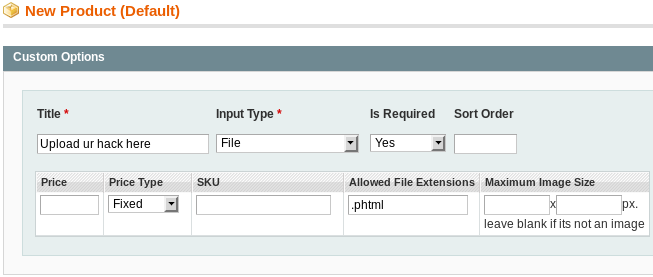
\includegraphics[width=\textwidth]{figures/new-product-upload.png}
	\caption{\emph{The way to add an upload form to a product page.}}
	\label{fig:37811.py}
\end{figure}

So, now that we have a way to upload our reverse shell PHP file to the server, we need to trick the server into executing it. The aforementioned blogpost does this via an XML trick.

Here I deviate from the blog post a little. In the used version of Magento I couldn't find the mentioned `design tab' on the product page, so I started to look for other ways that I could give custom \verb|Layout Update XML|. I found that creating new page\footnote{\verb|CMS > Pages|} also provided the option to give custom XML\footnote{\verb|CMS > Pages > New Page > Design > Page Layout|}.

Then I had to figure out where the uploaded \verb|.phtml| file actually was placed on the filesystem. I made a guess that it'd be the default installation, so \verb|/var/www/html|. This was correct, and I obtained my reverse shell using \\\verb|nc -v -n -l -p 10365|.

\vspace{5mm}

However, then disaster struck. I had obtained the reverse shell, but after I submitted the user flag, I had left it alone. I hadn't documented the exact XML I used, and the server was reset by someone else. I had lost my reverse shell. I tried to do every step again, but I couldn't get it to work again. To this day I have no clue what was different in that specific instance of the server. I suspect another user had already changed some settings, which allowed this hack to work.

\begin{figure}[H]
	\centering
	\captionsetup{justification=centering}
	\noindent 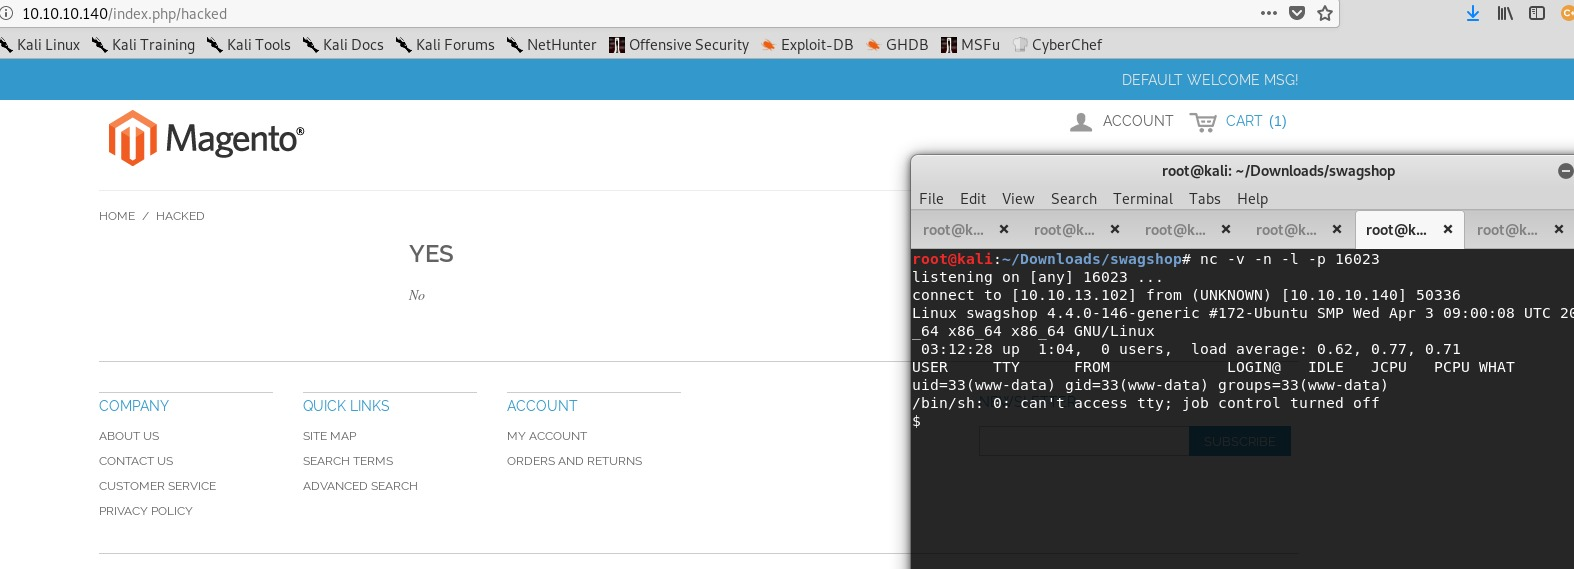
\includegraphics[width=\textwidth]{figures/exploit-1.jpeg}
	\caption{\emph{Screenshot of the initial shell I obtained.}}
	\label{fig:exploit1}
\end{figure}